\chapter{Frequently Asked Questions}
\label{faq}

\section{General Questions}

\subsection{What is Event-B?}
\index{Event-B}

Event-B is a formal method for system-level modelling and analysis. Key features of event-B are the use of set theory as a modelling notation, the use of refinement to represent systems at different abstraction levels and the use of mathematical proof to verify consistency between refinement levels.
More details are available in \url{http://www.event-b.org}.

\subsection{What is the difference between Event-B and the B method?}

Event-B (Section \ref{tut_eventb}) is derived from the \href{http://en.wikipedia.org/wiki/B-Method}{B method}. Both notations have the same \href{http://en.wikipedia.org/wiki/Jean-Raymond_Abrial}{inventor}, and share many common concepts (set-theory, refinement, proof obligations, ...) However, they are used for quite different purposes. The B method is devoted to the development of \textit{correct by construction} software, while the purpose of Event-B is used to model full systems (including hardware, software and environment of operation).

Event-B and the B method use mathematical languages which are similar but do not match exactly (in particular, operator precedences are different).

\subsection{What is Rodin?}
\index{Rodin}

The \textbf{Rodin Platform} is an Eclipse-based IDE for Event-B that provides support for refinement and mathematical proofs. The platform is open source, contributes to the Eclipse framework and can be extended with plugins.

\subsection{Where does the Rodin name come from?}

The Rodin Platform (Section \ref{rodin_platform}) was initially developed within the European Commission funded Rodin project (IST-511599 ), where Rodin is an acronym for ``Rigorous Open Development Environment for Complex Systems”. Rodin is also the name of a famous French sculptor. One of his most famous works is the \href{http://en.wikipedia.org/wiki/The_Thinker}{Thinker}. 

\subsection{Where I can download Rodin?}
\label{faq_where_download_rodin}

Rodin is available for download at the Rodin Download page: \url{http://wiki.event-b.org/index.php/Rodin_Platform_Releases}

\subsection{How to contribute and develop?}

Glad to hear that you want to help!  Please see the \url{http://wiki.event-b.org/index.php/Developer_FAQ} page.

\subsection{My operating system is not supported!  How can I install Rodin on my platform?}
\label{faq_os_not_supported}
At the time of this writing, prebuild versions only a small number of operating systems.  There are two recommended approaches for running Rodin in those situations:
\begin{description}
	\item[Build Rodin from the sources] For users who have some experience in building Java software, they may simply build Rodin from the sources.  For more information, please consult the Developer Documentation in the Rodin Wiki: \url{http://wiki.event-b.org/index.php/Rodin_Developer_Support}
	\item[Run Rodin in a virtual environment] With a fast computer, you can also use a virtual environment (e.g. VirtualBox) and install an operating system into that environment that supports Rodin (e.g. a 32bit version of Linux).
\end{description}

There are other options available for more specialized scenarios (e.g. running 32bit Rodin on a 64bit Linux system).  However, the two approaches outlined above are the least painful ones.

\section{General Tool Usage}

\subsection{Do I lose my proofs when I clean a project?}
\index{project!clean}
No! This is a common misunderstanding of what a project clean does. A project contains two kinds of files: 

\begin{itemize}
	\item those you can edit: contexts, machines, proofs 
	\item those generated by a project build: proof obligations, proof statuses (for each proof obligation, discharged or not discharged) 
\end{itemize}

The cleaner just undoes what the builder does, i.e. it removes proof obligations and statuses, but it never modifies any proof.

A status may change from \emph{discharged} to \emph{not discharged} when the proof is no longer compatible with the corresponding proof obligation (e.g. when a hypothesis is changed), but \textbf{the proof itself is still there!}
You can try to \href{http://wiki.event-b.org/index.php/Proof_Obligation_Commands#Proof_Replay_on_Undischarged_POs}{replay} it.

Confusion may arise when automatic provers have been launched. The cleaner does not undo these automatic proofs (why would it ?!!). Once a proof is made, the platform does not modify or delete it by itself. Even \href{http://wiki.event-b.org/index.php/Proof_Purger_Interface#Why_proofs_become_obsolete}{obsolete} proofs are preserved!

\subsection{How do I install external plugins without using Eclipse Update Manager?}

Although it is recommended that you install additional plugins into the Rodin platform using the Update Manager of Eclipse, this might not always be practical. In this case, you can install these plugins by emulating the operations normally performed by the Update Manager either manually or by using ad-hoc scripts. 

The manual installation of plugins is described in \href{http://wiki.event-b.org/index.php/Installing_external_plugins_manually}{\emph{Installing external plugins manually}}. 

\subsection{The builder takes too long}

Generally, the builder spends most of its time attempting to prove POs. There are basically two ways to get it out of the way: 

\begin{itemize}
	\item the first one is to disable the automated prover in the \textsf{Preferences} panel. 
	\item the second one is to mark a PO as reviewed if you do not want the auto-prover to attempt it anymore. 
\end{itemize}

Note that if you disable the automated prover, you always can run it later on some files by using the contextual menu in the Event-B Explorer. 

To disable the automated prover, open \textsf{Rodin Preferences} 
(menu \textsf{Window $\rangle$ Preferences...}). In the tree on the left-hand panel, select \textsf{Event-B $\rangle$ Sequent Prover $\rangle$ Auto-tactic}. Then, in the right-hand panel ensure that the checkbox labelled \textsf{Enable auto-tactic} for proving is disabled. 

To review a proof obligation, just open it in the interactive prover and then click on the \emph{review} button (this is a round blue button with a \emph{R} in the proof control toolbar). The proof obligation should now labelled with the same icon in the Event-B explorer. 

\subsection{What are the ASCII shortcuts for mathematical operators}
\index{symbols}

The ASCII shortcuts that can be used for entering mathematical operators are described in the following section: \textsf{Rodin Keyboard User Guide $\rangle$ Getting Started $\rangle$ Special Combos}. 

This page is also available in the dynamic help system. The advantage of using dynamic help is that it is able to display the help page side-by-side with the other views and editors. To start the dynamic help, click \textsf{Help $\rangle$ Dynamic Help}, then click \textsf{All Topics} and select the page in the tree. 

\subsection{Rodin (and Eclipse) doesn't take into account the MOZILLA\_FIVE\_HOME environment variable}

You have to add a property by appending the following code to your \textsf{eclipse/eclipse.ini} or \textsf{rodin/rodin.ini} file: 

\begin{verbatim} 
	-Dorg.eclipse.swt.browser.XULRunnerPath=/usr/lib/xulrunner/xulrunner-xxx 
\end{verbatim} 

\subsection{No More Handles}

On Windows platforms, it may happen that Rodin crashes, complaining that there are ``no more handles''. This is an OS specific limitation, described \href{http://journals.jevon.org/users/jevon-phd/entry/19833}{here} and \href{https://bugs.eclipse.org/bugs/show_bug.cgi?id=211124}{there}. A workaround is provided at \href{http://blogs.msdn.com/b/ntdebugging/archive/2007/01/04/desktop-heap-overview.aspx}{this site}. 

\subsection{Software installation fails}

The installation of software from update sites (\textsf{Help $\rangle$ Install New Software...}) sometimes fails with an error saying something like: 

\begin{verbatim}
No repository found containing: osgi.bundle,org.eclipse.emf.compare,1.0.1.v200909161031
No repository found containing: osgi.bundle,org.eclipse.emf.compare.diff,1.0.1.v200909161031
...
\end{verbatim}

This is an eclipse/p2 bug, referenced \href{http://stackoverflow.com/questions/511367/error-when-updating-eclipse}{here}. 

The workaround is to: 

\begin{itemize}
	\item Go to \textsf{Window $\rangle$ Preferences $\rangle$ Install/Update $\rangle$ Available Software Sites} 
	\item Remove all sites then add them back again, which can be achieved in the \textsf{Available Software Sites} preference page by: 
	\item Select all update sites (by highlighting them all those that are checked) 
	\item Export them 
	\item Remove them
	\item Restart Rodin
	\item Go back to the preference page and import update sites back (from the previously exported file) 
\end{itemize}

\section{Modeling}
\index{modeling}

\subsection{Witness for \textsf{Xyz} missing. Default witness generated}

A parameter has disappeared during a refinement. If this is intentional, you have to add a witness \ref{witness} telling how the abstract parameter is refined. 

\subsection{Identifier \textsf{Xyz} should not occur free in a witness}

You refer to \textsf{Xyz} in a witness predicate where \textsf{Xyz} is a disappearing abstract variable or parameter which is not set as the witness label. 

\subsection{In \textsf{INITIALISATION}, I get Witness \textsf{Xyz} must be a disappearing abstract variable or parameter}
\index{witness}

The witness is for the after value of the abstract variable, hence you should use the primed variable. The witness label should be \textsf{Xyz'}, and the predicate should refer to \textsf{Xyz'} too. 

\subsection{I've added a witness for \textsf{Xyz} but it keeps saying ``Identifier \textsf{Xyz} has not been defined''}

As specified in the \ref{witness} section, the witness must be labelled by the name \textsf{Xyz} of the concrete variable being concerned.

\subsection{How can I create a new Event-B Project?}
\index{project}

Please check Tutorial \ref{tut_project_setup} to learn how to create a new Event-B project.

\subsection{How to remove a Event-B Project?}

In order to remove a project, first select it on the \textsf{Project Explorer} and then right click with the mouse. The contextual menu will appear on the screen as indicated in Figure \ref{fig_faq_removeproject}.

\begin{figure}[!ht]
\begin{center}
	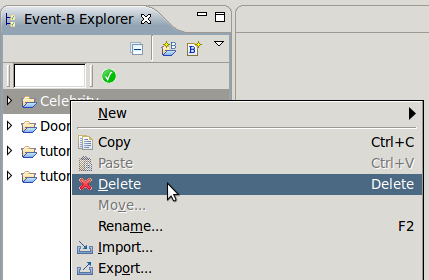
\includegraphics{img/faq/faq_removeproject.png}
	\caption{Removing a Event-B Project}
	\label{fig_faq_removeproject}
\end{center}
\end{figure}

You simply click on \textsf{Delete} and your project will be deleted (after you confirm it in the window that pops up). It is then removed from the \textsf{Project Explorer}.

\subsection{How to export an Event-B Project?}

Exporting a project is the operation by which you can construct automatically a ``zip" file containing the entire project. Such a file is ready to be sent by mail. Once received, an exported project can be imported (next section). It then becomes a project like the other ones which were created locally. In order to export a project, first select it, and then click on \textsf{File $\rangle$ Export...} from the menubar as indicated in Figure \ref{fig_faq_exportproject}. 

\begin{figure}[!ht]
\begin{center}
	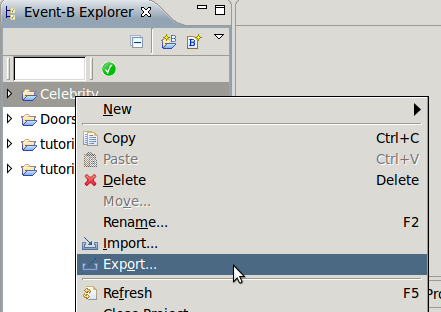
\includegraphics{img/faq/faq_exportproject.png}
	\caption{Export a Event-B Project}
	\label{fig_faq_exportproject}
\end{center}
\end{figure}

The Export wizard will pop up. In this window, select \textsf{General $\rangle$ Archive File} and click the \textsf{Next $>$} button. Specify the path and name of the archive file into which you want to export your project and finally click \textsf{Finish}. This menu sequence belongs to Eclipse (as well as the various options). For more information, refer to the Eclipse documentation. 

\subsection{How to import a Event-B Project?}

A ``.zip" file corresponding to a project which has been exported elsewhere can be imported locally. In order to do this, click on \textsf{File $\rangle$ Import} from the menubar. In the import wizard, select \textsf{General $\rangle$ Existing Projects into Workspace} and click \textsf{Next $>$}. Then, enter the file name of the imported project and finally click \textsf{Finish}. As with exporting, the menu sequence and layout are part of Eclipse.

The importation will fail if the name of the imported project (not the name of the file) is the same as the name of an existing local project. The moral of the story is that when exporting a project to a partner you need to modify its name in case your partner already has a project with that same name (which could be a previous version of the exported project). Changing the name of a project is explained in the next section. 

\subsection{How to change the name of a Event-B Project?}

Select the project whose name you want to modify, and then click on \textsf{File $\rangle$ Rename...}. Modify the name and click on \textsf{OK}. The name of your project will then have been modified accordingly. 

\subsection{How to create a Event-B Component}

Please check Tutorial \ref{tut_project_setup} to learn how to create a new Event-B component.

\subsection{How to remove a Event-B Component}

In order to remove a component, press the right mouse button on the component. In the context menu, select \textsf{Delete}. This component is removed from the \textsf{Project Explorer}. 

\subsection{In the new Rodin Editor, how can I add an element to machine?}
\label{faq_new_editor_new_element}

\info{Please also consult section~\label{new_eventb_editor}, which describes the editor.}

Whenever using the context menu of the new editor, please pay attention to the following two issues:
\begin{itemize}
	\item Make sure that the cursor already is on the correct line.  If you right-click and the cursor is on the wrong line, you will get an incorrect context menu.
	\item Make sure the cursor is not in ``edit'' mode, where you can edit a textual element.  In that scenario you will also get an incorrect context menu.
\end{itemize}

The different elements of the machine, can of course, be added using the different wizards for element creation (New Variable Wizard \icon{rodin/newvar_edit.png}, New Variant Wizard \icon{rodin/newvariant_edit.png}, New Invariant Wizard \icon{rodin/newinv_edit.png}, and New Event Wizard \icon{rodin/newevt_edit.png}) which are described in more detail in Chapter \ref{eventb_wizards}. 

You can also add new elements by placing your cursor directly to the left of the small green arrow that appears next to your machine name in \textsf{MACHINE} section. Now right click and select the component that you want to add from the \textsf{Add Child} menu. You can also add an element by right clicking on the heading of the section of the element you want to add (e.g. \textsf{VARIABLES}) and selecting \textsf{Add Child}, or by placing your directly to the left of the small green arrow next to the name of any of the components that already exist and selecting \textsf{Add Sibling}. Unfortunately, the if your cursor is not directly next to the small green arrow (while the cursor is blinking, the left side of the arrow is actually touching the cursor), these methods do not actually work. 

\subsection{How can I use multiple lines for a comment, predicate or expression (using the new editor)?}

To insert a linebreak while editing any field, use Ctrl-Return.

\subsection{How to save a Context or a Machine}

Once a machine or context is (partially) edited, you can save it by using the save button as indicated in Figure \ref{fig_faq_saveaction}.

\begin{figure}[!ht]
\begin{center}
	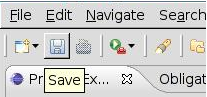
\includegraphics{img/faq/faq_saveaction.png}
	\caption{Save a context or a machine}
	\label{fig_faq_saveaction}
\end{center}
\end{figure}

Once a ``Save" is done, three tools are called automatically, these are:

\begin{itemize}
	\item the Static Checker
	\item the Proof Obligation Generator (Section \ref{generated_proof_obligations})
	\item the Auto-Prover (Section \ref{auto_prover})
\end{itemize}

This can some time. A ``Progress" window can be opened at the bottom right of the screen to see which tools are working (most of the time, it will be the auto-prover). 

\section{Proving}
\index{proving}

\subsection{Help!  Proving is difficult!}

Yes, it is.  Check out Section~\ref{use_provers_effectively} to get started with using the provers.

\subsection{How can I do a Proof by Induction?}

\href{http://wiki.event-b.org/index.php/Induction_proof}{This page about proof by induction} will give you some starting tips.

\subsection{Labels of proof tree nodes explained}

\begin{itemize}
	\item \textsf{ah} means \textit{add hypothesis},
	\item \textsf{eh} means rewrite with \textit{equality from hypothesis} from left to right,
	\item \textsf{he} means rewrite with \textit{equality from hypothesis} from right to left,
	\item \textsf{rv} tells us that this goal has been manually reviewed (see \ref{proof_control_view}),
	\item \textsf{sl/ds} means \textit{selection/deselection},
	\item \textsf{PP} means \textit{discharged by the predicate prover},
	\item \textsf{ML} means \textit{discharged by the mono lemma prover}
\end{itemize}

\section{Usage Questions}

\subsection{Where did the GUI window go?}

When you are looking for a particular view, and the view does not appear or if it appears in a different place than is usual, try clicking on \textsf{Window $\rangle $ Reset Perspective...}. This will reset the different views back to their default positions. If you can't find menu buttons from one of the views, try resizing the view in question to see if part of the menu has been hidden.

\subsection{Where vs. When: What's going on?}
\index{when}
\index{where}

You may have noticed that both in this tutorial, as well as in the tool, events sometimes use the keyword ``when'' and sometimes ``where''.  The idea of this was to make the formal statements more intuitive.  Unfortunately, this created more confusion than anything else.

The short answer is: ``when'' and ``where'' in events have exactly the same meaning, for all practical purposes.

The long answer is: In some contexts (but not all), the tool changes the keywords to make the meaning of the event more apparent.  The distinguishing factor is the parameter: Without parameter, ``when'' is used, with a parameter, ``where'' is used.

To confuse things even more, this doesn't apply everywhere: The structural editor always shows ``where'', but the pretty print toggles between the two.  The Event-B in this handbook has been generated with the \LaTeX plugin, which also toggles the keyword.

%%% Local Variables: 
%%% mode: latex
%%% TeX-master: "rodin-doc"
%%% End: 
